\documentclass[12pt,a4paper]{article}

% ─── Page Layout ───────────────────────────────────────────────────────────────
\usepackage[a4paper, margin=0.8in, headheight=14pt]{geometry}

% ─── Fonts (XeLaTeX) ───────────────────────────────────────────────────────────
\usepackage{fontspec}
\usepackage{unicode-math}
\setmainfont{TeX Gyre Pagella}
\setmonofont[Scale=0.88]{TeX Gyre Cursor}
\setmathfont{Latin Modern Math}

% ─── Packages ──────────────────────────────────────────────────────────────────
\usepackage{xcolor}
\usepackage{colortbl}
\usepackage{titlesec}
\usepackage{enumitem}
\usepackage{tabularx}
\usepackage{booktabs}
\usepackage{array}
\usepackage{amsmath}
\usepackage{tikz}
\usetikzlibrary{shapes.geometric, arrows.meta, positioning, calc, fit, decorations.pathreplacing}
\usepackage{tcolorbox}
\tcbuselibrary{skins, breakable}
\usepackage{hyperref}
\usepackage{fancyhdr}
\usepackage{graphicx}
\usepackage{microtype}
\hyphenpenalty=10000
\exhyphenpenalty=10000
\sloppy
\usepackage{caption}
\usepackage{setspace}
\usepackage{multirow}
\usepackage{tocloft}

% ─── Q&A helper ────────────────────────────────────────────────────────────────
\newcommand{\Q}[1]{\textbf{#1}\par\noindent\ignorespaces}

% ─── Colour Palette ────────────────────────────────────────────────────────────
\definecolor{myred}{RGB}{196,30,58}
\definecolor{mydark}{RGB}{30,30,50}
\definecolor{mygreen}{RGB}{14,120,80}
\definecolor{myteal}{RGB}{0,130,140}
\definecolor{myamber}{RGB}{180,100,0}
\definecolor{mypurple}{RGB}{100,30,160}
\definecolor{mygray}{RGB}{246,247,249}
\definecolor{mgframe}{RGB}{180,185,200}
\definecolor{watermark}{RGB}{145,150,170}
\definecolor{hdrred}{RGB}{250,232,235}
\definecolor{hdrgreen}{RGB}{220,244,233}
\definecolor{hdrteal}{RGB}{220,242,244}
\definecolor{hdramber}{RGB}{253,242,215}
\definecolor{hdrpurple}{RGB}{238,228,255}
\definecolor{hdrgray}{RGB}{238,240,245}
\definecolor{rowalt}{RGB}{250,251,253}

% ─── Section Formatting ────────────────────────────────────────────────────────
\titleformat{\section}
  {\large\bfseries\color{myred}}{\thesection.}{0.5em}{}
  [\vspace{1pt}{\color{myred}\rule{\linewidth}{0.8pt}}]
\titleformat{\subsection}
  {\normalsize\bfseries\color{myteal}}{\thesubsection}{0.5em}{}
\titlespacing*{\section}{0pt}{18pt}{7pt}
\titlespacing*{\subsection}{0pt}{11pt}{4pt}

% ─── Paragraph ─────────────────────────────────────────────────────────────────
\setlength{\parindent}{0pt}
\setlength{\parskip}{4pt}

% ─── TOC Styling ───────────────────────────────────────────────────────────────
\renewcommand{\cfttoctitlefont}{\large\bfseries\color{myred}}
\renewcommand{\cftaftertoctitle}{\par\noindent{\color{myred}\rule{\linewidth}{0.8pt}}}
\setlength{\cftbeforetoctitleskip}{0pt}
\setlength{\cftaftertoctitleskip}{6pt}
\renewcommand{\cftsecfont}{\normalsize\bfseries\color{mydark}}
\renewcommand{\cftsecpagefont}{\normalsize\bfseries\color{mydark}}
\renewcommand{\cftsecleader}{\cftdotfill{\cftdotsep}}
\setlength{\cftbeforesecskip}{7pt}
\renewcommand{\cftsubsecfont}{\small\color{mydark}}
\renewcommand{\cftsubsecpagefont}{\small\color{mydark}}
\setlength{\cftbeforesubsecskip}{3pt}
\setlength{\cftsubsecindent}{1.4em}

% ─── Table helpers ─────────────────────────────────────────────────────────────
\renewcommand{\arraystretch}{1.45}
\setlength{\tabcolsep}{6pt}
\arrayrulecolor{mydark}
\newcolumntype{B}[1]{>{\small\bfseries\raggedright\arraybackslash}m{#1}}
\newcolumntype{Y}{>{\small\raggedright\arraybackslash}X}
\renewcommand{\tabularxcolumn}[1]{m{#1}}

% ─── Header / Footer ───────────────────────────────────────────────────────────
\pagestyle{fancy}
\fancyhf{}
\fancyhead[L]{\small\color{myred}\textbf{PE-EC701C}\;\color{mydark}--- Mobile Communication and Networks}
\fancyhead[R]{\small\color{myteal}\textbf{Module 5 Notes}}
\fancyfoot[C]{\small\color{mydark}\thepage}
\fancyfoot[R]{\small\color{watermark}\textit{\copyright\ Biraj}}
\renewcommand{\headrulewidth}{0.5pt}
\renewcommand{\footrulewidth}{0.3pt}

% ─── Hyperref ──────────────────────────────────────────────────────────────────
\hypersetup{
  colorlinks=true, linkcolor=myteal, urlcolor=myteal,
  pdfauthor={Biraj Sarkar},
  pdftitle={PE-EC701C --- Module 5 Notes}
}

% ─── tcolorbox styles ──────────────────────────────────────────────────────────
\tcbset{
  tikzbox/.style={
    colback=mygray, colframe=mgframe, boxrule=0.6pt, arc=4pt,
    left=8pt, right=8pt, top=6pt, bottom=6pt,
    colbacktitle=mgframe, coltitle=mydark,
    fonttitle=\small\bfseries
  },
  defbox/.style={
    colback=hdrgreen, colframe=mygreen, boxrule=0.8pt, arc=4pt,
    left=9pt, right=9pt, top=6pt, bottom=6pt,
    colbacktitle=mygreen, coltitle=white,
    fonttitle=\small\bfseries
  },
  formulabox/.style={
    colback=hdrteal, colframe=myteal, boxrule=0.8pt, arc=4pt,
    left=9pt, right=9pt, top=7pt, bottom=7pt,
    colbacktitle=myteal, coltitle=white,
    fonttitle=\small\bfseries
  },
  examplebox/.style={
    colback=hdramber, colframe=myamber, boxrule=0.8pt, arc=4pt,
    left=9pt, right=9pt, top=6pt, bottom=6pt,
    colbacktitle=myamber, coltitle=white,
    fonttitle=\small\bfseries
  },
  masonbox/.style={
    colback=hdrpurple, colframe=mypurple, boxrule=0.8pt, arc=4pt,
    left=9pt, right=9pt, top=6pt, bottom=6pt,
    colbacktitle=mypurple, coltitle=white,
    fonttitle=\small\bfseries
  },
  exambox/.style={
    colback=hdrpurple, colframe=mypurple, boxrule=1pt, arc=5pt,
    left=10pt, right=10pt, top=8pt, bottom=8pt,
    colbacktitle=mypurple, coltitle=white,
    fonttitle=\bfseries,
    breakable, title after break={\textbf{Frequently Asked / Viva Questions (contd.)}}}
}
\tcbset{breakable}

% ─── TikZ styles ───────────────────────────────────────────────────────────────
\tikzset{
  block/.style={rectangle, draw=myteal, fill=hdrteal,
    text width=2.4cm, align=center, minimum height=0.95cm,
    font=\small, rounded corners=3pt, line width=0.7pt},
  redblock/.style={rectangle, draw=myred, fill=hdrred,
    text width=2.4cm, align=center, minimum height=0.95cm,
    font=\small, rounded corners=3pt, line width=0.7pt},
  netnode/.style={rectangle, draw=myteal, fill=hdrteal,
    text width=1.5cm, align=center, minimum height=0.8cm,
    font=\small, rounded corners=3pt, line width=0.7pt},
  sumjunc/.style={circle, draw=myamber, fill=hdramber,
    minimum size=0.62cm, font=\small, line width=0.8pt},
  snode/.style={circle, draw=mypurple, fill=hdrpurple,
    minimum size=0.55cm, font=\footnotesize, line width=0.7pt},
  arrow/.style={-Stealth, thick, color=mydark},
  redarrow/.style={-Stealth, thick, color=myred},
  line/.style={thick, color=mydark}
}

% ═══════════════════════════════════════════════════════════════════════════════
\begin{document}
% ═══════════════════════════════════════════════════════════════════════════════

\begin{center}
  {\LARGE\bfseries\color{myred} PE-EC701C --- Mobile Communication and Networks}\\[5pt]
  {\normalsize\color{mydark} Semester VII \quad$\bullet$\quad 3L:0T:0P \quad$\bullet$\quad 3 Credits}\\[3pt]
  {\normalsize\color{myteal}\textbf{Module 5 Exam Notes: Receiver Structure and Diversity Techniques}}\\[3pt]
  {\small\color{mydark} CGEC \;$|$\; B.Tech ECE (2023--27) \;$|$\; \textit{Biraj Sarkar}}
\end{center}
\noindent{\color{myred}\rule{\linewidth}{1.5pt}}
\vspace{2pt}

\hypersetup{linkcolor=mydark}
\tableofcontents
\hypersetup{linkcolor=myteal}
\newpage

% ===============================================================================
\section{Diversity Reception Concepts and Combining Methods}
% ===============================================================================

Fading causes severe degradation in signal quality. Diversity reception exploits the physical fact that if two or more independent signal paths can be established, the probability that all paths fade simultaneously is extremely low.

\begin{tcolorbox}[defbox]
\textbf{Diversity Reception:} A technique where a receiver is provided with multiple independent copies (channels) of the same transmitted signal, which are then combined to improve the overall Signal-to-Noise Ratio (SNR) and mitigate fading.
\end{tcolorbox}

\subsection{Types of Diversity Schemes}
\begin{itemize}[leftmargin=*, itemsep=3.0pt]
  \item \textbf{Space Diversity:} Employs multiple antennas spaced physically apart. For receive antennas, a spacing of $\approx 0.5\lambda$ at the mobile terminal or $10\lambda$ at the base station is sufficient to ensure uncorrelated fading.
  \item \textbf{Time Diversity:} Transmits the same signal in different time slots. The spacing between transmissions must be larger than the coherence time $T_c$ of the channel. Often implemented using channel coding and interleaving.
  \item \textbf{Frequency Diversity:} Transmits the same information on different carrier frequencies. The frequency spacing must exceed the coherence bandwidth $B_c$ of the channel.
  \item \textbf{Polarization Diversity:} Utilizes orthogonal polarization states (e.g., horizontal/vertical or $\pm 45^\circ$). Requires only a single antenna structure with dual-polarized elements, saving space.
\end{itemize}

\subsection{Diversity Combining Methods}
Let $M$ be the number of independent receive branches (diversity paths). Each branch receives a signal with envelope $r_i$ and noise power $\sigma_N^2$.
\begin{enumerate}[label=\textbf{\arabic*.}, leftmargin=*, itemsep=4.0pt]
  \item \textbf{Selection Combining (SC):} The receiver continuously monitors the SNR of all $M$ branches and selects the branch with the highest instantaneous SNR:
    \begin{equation}
      \gamma_{\text{out}} = \max(\gamma_1, \gamma_2, \dots, \gamma_M)
    \end{equation}
    It is simple to implement but does not exploit the signal energy of the other $M-1$ branches.
  \item \textbf{Maximal Ratio Combining (MRC):} The signals from all branches are co-phased (aligned in phase) and weighted proportionally to their individual signal voltage-to-noise power ratios before summing:
    \begin{equation}
      r_{\text{out}}(t) = \sum_{i=1}^{M} w_i r_i(t) \quad \text{where } w_i = \frac{r_i}{\sigma_N^2}
    \end{equation}
    The output SNR is the sum of the individual branch SNRs:
    \begin{equation}
      \gamma_{\text{out}} = \sum_{i=1}^{M} \gamma_i
    \end{equation}
    MRC is the optimal combining scheme, yielding the maximum possible SNR improvement.
  \item \textbf{Equal Gain Combining (EGC):} The signals are co-phased and summed with equal weights ($w_i = 1$):
    \begin{equation}
      r_{\text{out}}(t) = \sum_{i=1}^{M} r_i(t)
    \end{equation}
    EGC offers performance close to MRC but is less complex, as it does not require continuous estimation of branch signal amplitudes.
\end{enumerate}

\begin{tcolorbox}[tikzbox, title={Maximal Ratio Combining (MRC) Block Diagram}]
\centering
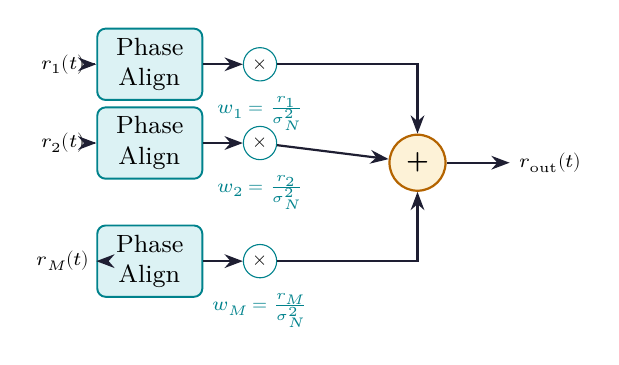
\begin{tikzpicture}[node distance=0.6cm and 1.0cm, every node/.style={font=\scriptsize}]
  % Inputs
  \node (r1) at (0, 1.5) {$r_1(t)$};
  \node (r2) at (0, 0.5) {$r_2(t)$};
  \node (rM) at (0, -1.0) {$r_M(t)$};
  \node at (0, -0.25) {\vdots};

  % Weight multipliers
  \node[circle, draw=myteal, inner sep=2pt] (m1) at (2.5, 1.5) {$\times$};
  \node[circle, draw=myteal, inner sep=2pt] (m2) at (2.5, 0.5) {$\times$};
  \node[circle, draw=myteal, inner sep=2pt] (mM) at (2.5, -1.0) {$\times$};

  % Weight labels below multipliers
  \node[below=2pt of m1, color=myteal] {$w_1 = \frac{r_1}{\sigma_N^2}$};
  \node[below=2pt of m2, color=myteal] {$w_2 = \frac{r_2}{\sigma_N^2}$};
  \node[below=2pt of mM, color=myteal] {$w_M = \frac{r_M}{\sigma_N^2}$};

  % Phase adjusters (in-between)
  \node[block, text width=1.1cm, minimum height=0.6cm] (p1) at (1.1, 1.5) {Phase\\Align};
  \node[block, text width=1.1cm, minimum height=0.6cm] (p2) at (1.1, 0.5) {Phase\\Align};
  \node[block, text width=1.1cm, minimum height=0.6cm] (pM) at (1.1, -1.0) {Phase\\Align};

  % Summation
  \node[sumjunc] (sum) at (4.5, 0.25) {\textbf{+}};
  \node[right=0.8cm of sum] (out) {$r_{\text{out}}(t)$};

  % Connections
  \draw[arrow] (r1) -- (p1); \draw[arrow] (p1) -- (m1);
  \draw[arrow] (r2) -- (p2); \draw[arrow] (p2) -- (m2);
  \draw[arrow] (rM) -- (pM); \draw[arrow] (pM) -- (mM);

  \draw[arrow] (m1) -| (sum);
  \draw[arrow] (m2) -- (sum);
  \draw[arrow] (mM) -| (sum);
  
  \draw[arrow] (sum) -- (out);
\end{tikzpicture}
\end{tcolorbox}

% ===============================================================================
\section{RAKE Receiver}
% ===============================================================================

In wideband CDMA systems, the signal bandwidth is larger than the coherence bandwidth of the channel, making the channel frequency-selective. This time dispersion resolved as distinct multipath components is exploited by the RAKE receiver.

\begin{tcolorbox}[defbox]
\textbf{RAKE Receiver:} A receiver designed for spread-spectrum CDMA systems that uses multiple parallel correlators called \textbf{fingers} to independently track, delay-align, and combine individual multipath components, turning time dispersion into a source of diversity.
\end{tcolorbox}

\subsection{Working Principle}
\begin{itemize}[leftmargin=*, itemsep=3.0pt]
  \item \textbf{Resolution:} The chip duration ($T_c$) of a CDMA code is very short. If the difference in propagation delay between two paths is greater than $T_c$, the receiver can resolve them as independent paths.
  \item \textbf{Fingers:} The RAKE receiver allocates one "finger" to each resolved multipath component. Each finger correlates the received signal with a delayed version of the spreading code $c(t - \tau_i)$ corresponding to that path's excess delay $\tau_i$.
  \item \textbf{Combining:} The outputs of all fingers are co-phased and combined using Maximal Ratio Combining (MRC).
\end{itemize}

\begin{tcolorbox}[tikzbox, title={RAKE Receiver Finger Structure}]
\centering
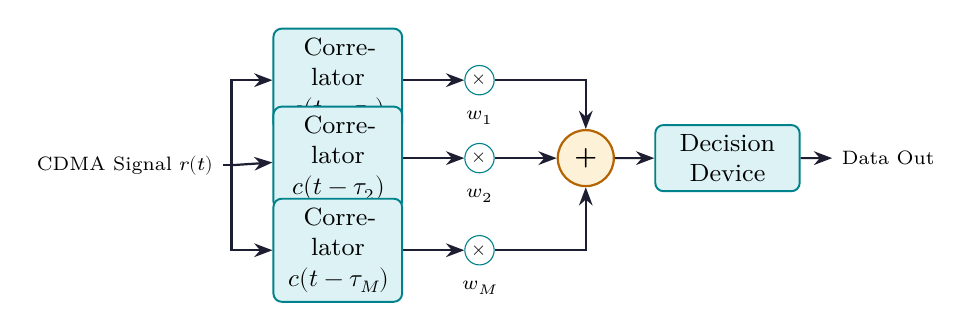
\begin{tikzpicture}[scale=0.9, every node/.style={font=\scriptsize}]
  % Input
  \node (in) at (-1, 0) {CDMA Signal $r(t)$};

  % Split into fingers
  \node[block, text width=1.4cm, minimum height=0.7cm] (cor1) at (2, 1.2) {Correlator\\$c(t-\tau_1)$};
  \node[block, text width=1.4cm, minimum height=0.7cm] (cor2) at (2, 0.1) {Correlator\\$c(t-\tau_2)$};
  \node[block, text width=1.4cm, minimum height=0.7cm] (corM) at (2, -1.2) {Correlator\\$c(t-\tau_M)$};

  % Multipliers
  \node[circle, draw=myteal, inner sep=1.5pt] (m1) at (4.0, 1.2) {$\times$};
  \node[circle, draw=myteal, inner sep=1.5pt] (m2) at (4.0, 0.1) {$\times$};
  \node[circle, draw=myteal, inner sep=1.5pt] (mM) at (4.0, -1.2) {$\times$};

  \node[below=2pt of m1] {$w_1$};
  \node[below=2pt of m2] {$w_2$};
  \node[below=2pt of mM] {$w_M$};

  % Summation
  \node[sumjunc] (sum) at (5.5, 0.1) {\textbf{+}};
  \node[block, right=0.5cm of sum, text width=1.6cm, minimum height=0.7cm] (det) {Decision\\Device};
  \node[right=0.4cm of det] (out) {Data Out};

  % Connect lines
  \draw[line] (in) -- (0.5, 0);
  \draw[arrow] (0.5, 0) |- (cor1);
  \draw[arrow] (0.5, 0) -- (cor2);
  \draw[arrow] (0.5, 0) |- (corM);

  \draw[arrow] (cor1) -- (m1);
  \draw[arrow] (cor2) -- (m2);
  \draw[arrow] (corM) -- (mM);

  \draw[arrow] (m1) -| (sum);
  \draw[arrow] (m2) -- (sum);
  \draw[arrow] (mM) -| (sum);

  \draw[arrow] (sum) -- (det);
  \draw[arrow] (det) -- (out);
\end{tikzpicture}
\end{tcolorbox}

% ===============================================================================
\section{Channel Equalization}
% ===============================================================================

Equalizers combat Inter-Symbol Interference (ISI) caused by time-dispersive fading channels by modeling the inverse of the channel's transfer function.

\subsection{Linear Equalizers}
Linear equalizers process the received signal using a linear transversal filter (Tapped Delay Line):
\begin{enumerate}[label=\textbf{\arabic*.}, leftmargin=*, itemsep=3.5pt]
  \item \textbf{Zero-Forcing Equalizer (ZFE):} Forces the equalizer output to have zero ISI at the decision points. Its frequency response is the exact inverse of the channel response:
    \begin{equation}
      H_{\text{eq}}(f) = \frac{1}{H(f)}
    \end{equation}
    \textbf{Limitation:} In spectral nulls (frequencies where the channel gain $H(f)$ is very small), ZFE heavily amplifies the noise.
  \item \textbf{Minimum Mean Square Error (MMSE) Equalizer:} Minimizes the mean square error between the actual transmitted symbol and the equalizer output, providing a balance between ISI mitigation and noise amplification:
    \begin{equation}
      H_{\text{eq}}(f) = \frac{H^*(f)}{|H(f)|^2 + \frac{N_0}{E_s}}
    \end{equation}
\end{enumerate}

\subsection{Adaptive Equalizers}
Since mobile channels are time-varying, the equalizer coefficients must adapt dynamically.
\begin{itemize}[leftmargin=*, itemsep=3.0pt]
  \item \textbf{LMS (Least Mean Squares) Algorithm:} A gradient-descent optimization algorithm that adjusts coefficients iteratively to minimize the mean square error. It is simple to implement but has a slow convergence rate.
  \item \textbf{RLS (Recursive Least Squares) Algorithm:} A more complex algorithm that utilizes least-squares estimation to update weights. It converges much faster than LMS but has significantly higher computational complexity.
\end{itemize}

\subsection{Non-linear Equalizers (Decision Feedback Equalizer - DFE)}
When the channel has severe spectral nulls, linear equalizers perform poorly due to noise amplification. Non-linear equalizers solve this:
\begin{itemize}[leftmargin=*, itemsep=3.0pt]
  \item \textbf{DFE Structure:} Consists of a \textbf{Feedforward Filter} (similar to a linear equalizer) and a \textbf{Feedback Filter}.
  \item \textbf{Feedback Mechanism:} The feedback filter takes previously decided symbols, reconstructs the resulting ISI, and subtracts it from the current input before the decision device. Because the subtracted ISI is based on clean decided symbols, it introduces no noise amplification.
\end{itemize}

% ===============================================================================
\section{Transmit Diversity and the Alamouti Scheme}
% ===============================================================================

Transmit diversity shifts the complexity of multiple antennas from the mobile terminal (downlink receiver) to the base station (downlink transmitter).

\subsection{The Alamouti Scheme (2x1 MIMO)}
The Alamouti scheme is a simple and elegant space-time block coding (STBC) method that achieves a diversity order of 2 using two transmit antennas ($Tx_0, Tx_1$) and one receive antenna ($Rx$).

\begin{tcolorbox}[tikzbox, title={Alamouti 2x1 Transmit Diversity Configuration}]
\centering
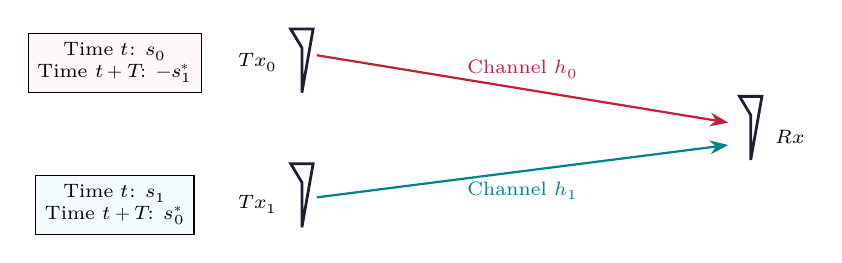
\begin{tikzpicture}[scale=0.95, every node/.style={font=\scriptsize}]
  % Transmit Antennas
  \draw[line, line width=1pt] (0, 1.2) -- (0, 1.8) -- (-0.15, 2.05) -- (0.15, 2.05) -- cycle;
  \node[left] at (-0.2, 1.6) {$Tx_0$};
  
  \draw[line, line width=1pt] (0, -0.6) -- (0, 0.0) -- (-0.15, 0.25) -- (0.15, 0.25) -- cycle;
  \node[left] at (-0.2, -0.3) {$Tx_1$};

  % Receiver Antenna
  \draw[line, line width=1pt] (6, 0.3) -- (6, 0.9) -- (5.85, 1.15) -- (6.15, 1.15) -- cycle;
  \node[right] at (6.2, 0.6) {$Rx$};

  % Channel lines
  \draw[arrow, color=myred] (0.2, 1.7) -- (5.7, 0.8) node[midway, above] {Channel $h_0$};
  \draw[arrow, color=myteal] (0.2, -0.2) -- (5.7, 0.5) node[midway, below] {Channel $h_1$};

  % Space-Time mapping tables
  \node[draw, fill=hdrred!30, align=center] at (-2.5, 1.6) {Time $t$: $s_0$\\Time $t+T$: $-s_1^*$};
  \node[draw, fill=hdrteal!30, align=center] at (-2.5, -0.3) {Time $t$: $s_1$\\Time $t+T$: $s_0^*$};
\end{tikzpicture}
\end{tcolorbox}

\subsection{Space-Time Block Coding Matrix and Derivation}
The transmit scheme maps two symbols $s_0$ and $s_1$ over two symbol periods ($t$ and $t+T$):
\par\noindent
\begin{tabularx}{\linewidth}{|B{3.2cm}|Y|Y|}
\hline
\rowcolor{hdrgray}
\textbf{Antenna / Time} & \textbf{Time $t$} & \textbf{Time $t+T$} \\
\hline
\textbf{Antenna $Tx_0$} & $s_0$ & $-s_1^*$ \\
\hline
\rowcolor{rowalt}
\textbf{Antenna $Tx_1$} & $s_1$ & $s_0^*$ \\
\hline
\end{tabularx}

Let $h_0$ and $h_1$ be the complex channel gains from $Tx_0$ and $Tx_1$ to the receive antenna, assumed constant over both symbol periods. The received signals $r_0$ and $r_1$ are:
\begin{equation}
  r_0 = r(t) = h_0 s_0 + h_1 s_1 + n_0
\end{equation}
\begin{equation}
  r_1 = r(t+T) = -h_0 s_1^* + h_1 s_0^* + n_1
\end{equation}
Where $n_0, n_1$ are AWGN noise terms. Taking the conjugate of $r_1$:
\begin{equation}
  r_1^* = -h_0^* s_1 + h_1^* s_0 + n_1^*
\end{equation}
We can write this in matrix form:
\begin{equation}
  \begin{bmatrix} r_0 \\ r_1^* \end{bmatrix} = \begin{bmatrix} h_0 & h_1 \\ h_1^* & -h_0^* \end{bmatrix} \begin{bmatrix} s_0 \\ s_1 \end{bmatrix} + \begin{bmatrix} n_0 \\ n_1^* \end{bmatrix}
\end{equation}
Let $\mathbf{H}_{\text{eff}} = \begin{bmatrix} h_0 & h_1 \\ h_1^* & -h_0^* \end{bmatrix}$ be the effective channel matrix. The columns of $\mathbf{H}_{\text{eff}}$ are orthogonal:
\begin{equation}
  \mathbf{H}_{\text{eff}}^H \mathbf{H}_{\text{eff}} = \left( |h_0|^2 + |h_1|^2 \right) \mathbf{I}_2
\end{equation}
The receiver decodes the symbols by multiplying the received vector by $\mathbf{H}_{\text{eff}}^H$:
\begin{equation}
  \begin{bmatrix} \tilde{s}_0 \\ \tilde{s}_1 \end{bmatrix} = \mathbf{H}_{\text{eff}}^H \begin{bmatrix} r_0 \\ r_1^* \end{bmatrix} = \begin{bmatrix} h_0^* r_0 + h_1 r_1^* \\ h_1^* r_0 - h_0 r_1^* \end{bmatrix}
\end{equation}
Expanding for symbol $s_0$:
\begin{equation}
  \tilde{s}_0 = \left( |h_0|^2 + |h_1|^2 \right) s_0 + h_0^* n_0 + h_1 n_1^*
\end{equation}
This yields an exact diversity order of 2, equivalent to 1x2 MRC at the receiver, but implemented at the transmitter.

% ===============================================================================
% MANDATORY QUICK REVISION PAGE
% ===============================================================================
\newpage
\begin{center}
  {\large\bfseries\color{myred} Quick Revision --- Module V}\\[3pt]
  {\small\color{mydark} Receiver Structure and Diversity Techniques $|$ PE-EC701C}
\end{center}
\noindent{\color{myred}\rule{\linewidth}{1.2pt}}
\vspace{4pt}

\begin{tcolorbox}[formulabox, title={\textbf{Key Formulas at a Glance}}]
\renewcommand{\arraystretch}{1.3}
\begin{tabularx}{\linewidth}{B{5.5cm} X}
Selection Combining (SC) SNR & $\gamma_{\text{out}} = \max(\gamma_1, \gamma_2, \dots, \gamma_M)$ \\
Maximal Ratio Combining (MRC) SNR & $\gamma_{\text{out}} = \sum_{i=1}^{M} \gamma_i$ \\
Linear Equalizer Output & $\hat{d}_k = \sum c_n y_{k-n}$ \\
Zero-Forcing Filter Relation & $H_{\text{eq}}(f) = \frac{1}{H(f)}$ \\
MMSE Filter Relation & $H_{\text{eq}}(f) = \frac{H^*(f)}{|H(f)|^2 + N_0/E_s}$ \\
Alamouti Matrix Orthogonality & $\mathbf{H}_{\text{eff}}^H \mathbf{H}_{\text{eff}} = \left( |h_0|^2 + |h_1|^2 \right) \mathbf{I}_2$ \\
Alamouti Decoded Symbol & $\tilde{s}_0 = h_0^* r_0 + h_1 r_1^*$
\end{tabularx}
\end{tcolorbox}

\begin{tcolorbox}[defbox, title={\textbf{One-Line Definitions}}]
\begin{itemize}[leftmargin=*, itemsep=2.5pt, topsep=0pt]
  \item \textbf{Selection Combining:} Diversity method selecting the single branch with the highest instantaneous SNR.
  \item \textbf{Maximal Ratio Combining:} Optimal combining method that co-phases and weights branches by their signal-to-noise ratio.
  \item \textbf{RAKE Receiver:} A CDMA receiver utilizing multiple correlator fingers to combine resolved multipath components.
  \item \textbf{Zero-Forcing Equalizer:} A linear equalizer that inverts the channel response, completely eliminating ISI at the cost of noise amplification.
  \item \textbf{DFE:} Decision Feedback Equalizer, a non-linear equalizer that subtracts the ISI of previously decided symbols.
  \item \textbf{Alamouti Scheme:} A 2x1 transmit diversity scheme mapping symbols over space and time using orthogonal block codes.
  \item \textbf{Space-Time Block Code:} Mapping data streams over multiple antennas and time slots to achieve transmit diversity.
\end{itemize}
\end{tcolorbox}

\begin{tcolorbox}[exambox, title={\textbf{Frequently Asked / Viva Questions}}]
\begin{enumerate}[topsep=0pt, label=\textbf{Q\arabic*.}, itemsep=5pt]
  \item \Q{Compare Selection Combining (SC) and Maximal Ratio Combining (MRC).}
    SC selects only the single branch with the highest instantaneous SNR. MRC co-phases and sums all branches weighted by their SNRs, maximizing performance by summing all signal energies.
  \item \Q{What is a RAKE receiver? Why is it named after a rake?}
    It is a CDMA receiver that resolves multipath components using parallel correlator fingers. It is named after a garden rake because it "rakes" together scattered multipath energies into a single coherent signal.
  \item \Q{Explain the noise amplification problem in Zero-Forcing Equalizers.}
    ZFE completely inverts the channel frequency response ($H_{\text{eq}} = 1/H(f)$). In deep channel fades (spectral nulls), $H(f) \to 0$, causing $H_{\text{eq}}$ to become extremely large, amplifying the background noise.
  \item \Q{Why does a Decision Feedback Equalizer (DFE) avoid noise amplification?}
    It uses a feedback filter to subtract the ISI caused by previously detected symbols. Because the feedback signal is derived from clean decided symbols rather than the noisy received signal, it introduces no noise.
  \item \Q{Derive the effective channel matrix and prove orthogonality in the Alamouti scheme.}
    $\mathbf{H}_{\text{eff}} = \begin{bmatrix} h_0 & h_1 \\ h_1^* & -h_0^* \end{bmatrix}$. Multiplying by its conjugate transpose: $\mathbf{H}_{\text{eff}}^H \mathbf{H}_{\text{eff}} = \begin{bmatrix} h_0^* & h_1 \\ h_1^* & -h_0 \end{bmatrix} \begin{bmatrix} h_0 & h_1 \\ h_1^* & -h_0^* \end{bmatrix} = \begin{bmatrix} |h_0|^2+|h_1|^2 & 0 \\ 0 & |h_0|^2+|h_1|^2 \end{bmatrix} = (|h_0|^2+|h_1|^2)\mathbf{I}_2$.
  \item \Q{State the antenna spacing requirements for space diversity.}
    To ensure uncorrelated fading, the spacing should be at least $0.5\lambda$ at the mobile terminal (due to rich local scattering) and $10\lambda$ to $20\lambda$ at the base station (due to high elevation and narrow angle of arrival).
  \item \Q{What are the advantages of polarization diversity over spatial diversity?}
    Polarization diversity uses orthogonal states (e.g. $\pm 45^\circ$) on a single physical antenna structure. It requires no physical spacing between antennas, saving base station tower space.
  \item \Q{What is the difference between LMS and RLS adaptive algorithms?}
    LMS uses a gradient-descent approach; it is simple but converges slowly. RLS uses recursive least-squares; it has high computational complexity but converges much faster.
  \item \Q{Explain the physical meaning of "co-phasing" in diversity combining.}
    Fading introduces independent phase shifts on each branch. Before summing the signals, the receiver must align their phases to prevent destructive interference (phase cancellation).
  \item \Q{Under what condition can a RAKE receiver resolve multipath components?}
    The delay difference between the multipath components must exceed the CDMA chip duration ($|\tau_1 - \tau_2| > T_c$). Otherwise, the paths cannot be separated.
  \item \Q{What is Equal Gain Combining (EGC)?}
    A combining method where branch signals are co-phased and summed with equal weights ($w_i=1$). It avoids the complex circuitry required to estimate signal amplitudes.
  \item \Q{Why is transmit diversity preferred over receive diversity in downlink design?}
    Adding multiple antennas to a mobile terminal increases its size, cost, and power consumption. Transmit diversity achieves similar performance gains by putting the multiple antennas on the base station.
\end{enumerate}
\tcbset{colbacktitle=myteal, coltitle=white}
\end{tcolorbox}

\begin{tcolorbox}[tikzbox, title={Comparison of Diversity Combining Methods}]
\renewcommand{\arraystretch}{1.4}
\par\noindent
\begin{tabularx}{\linewidth}{|B{3.0cm}|Y|Y|Y|}
\hline
\rowcolor{hdrgray}
\textbf{Parameter} & \textbf{Selection Combining} & \textbf{Equal Gain} & \textbf{Maximal Ratio} \\
\hline
\textbf{Logic} & Selects highest SNR branch. & Co-phases and sums equally. & Co-phases and weights by SNR. \\
\hline
\textbf{Complexity} & Low (no phase tracking needed). & Medium (requires co-phasing only). & High (requires phase and amplitude tracking). \\
\rowcolor{rowalt}
\hline
\textbf{Performance} & Lowest SNR gain. & Close to MRC ($\approx 1$ dB loss). & Optimal SNR gain. \\
\hline
\end{tabularx}
\tcbset{colbacktitle=myteal, coltitle=white}
\end{tcolorbox}

\end{document}
